%%%%%%%%%%%%%%%%%%%%%%%%%%%%%%%%%%%%%%%%%
% Journal Article
% LaTeX Template
% Version 1.4 (15/5/16)
%
% This template has been downloaded from:
% http://www.LaTeXTemplates.com
%
% Original author:
% Frits Wenneker (http://www.howtotex.com) with extensive modifications by
% Vel (vel@LaTeXTemplates.com)
%
% License:
% CC BY-NC-SA 3.0 (http://creativecommons.org/licenses/by-nc-sa/3.0/)
%
%%%%%%%%%%%%%%%%%%%%%%%%%%%%%%%%%%%%%%%%%

%----------------------------------------------------------------------------------------
%	PACKAGES AND OTHER DOCUMENT CONFIGURATIONS
%----------------------------------------------------------------------------------------

\documentclass[twoside,twocolumn]{article}

\usepackage{blindtext} % Package to generate dummy text throughout this template 

\usepackage[sc]{mathpazo} % Use the Palatino font
\usepackage[T1]{fontenc} % Use 8-bit encoding that has 256 glyphs
\linespread{1.05} % Line spacing - Palatino needs more space between lines
\usepackage{microtype} % Slightly tweak font spacing for aesthetics
\usepackage{graphicx}
\usepackage[english]{babel} % Language hyphenation and typographical rules
\usepackage{amsmath}
\usepackage[hmarginratio=1:1,top=32mm,columnsep=20pt]{geometry} % Document margins
\usepackage[hang, small,labelfont=bf,up,textfont=it,up]{caption} % Custom captions under/above floats in tables or figures
\usepackage{booktabs} % Horizontal rules in tables

\usepackage{lettrine} % The lettrine is the first enlarged letter at the beginning of the text
\usepackage[
backend=biber,
style=authoryear,
]{biblatex}
\title{A bibLaTeX example}
\addbibresource{tellis.bib} %Import the bibliography file

\usepackage{enumitem} % Customized lists
\setlist[itemize]{noitemsep} % Make itemize lists more compact

\usepackage{abstract} % Allows abstract customization
\renewcommand{\abstractnamefont}{\normalfont\bfseries} % Set the "Abstract" text to bold
\renewcommand{\abstracttextfont}{\normalfont\small\itshape} % Set the abstract itself to small italic text

\usepackage{titlesec} % Allows customization of titles
\renewcommand\thesection{\Roman{section}} % Roman numerals for the sections
\renewcommand\thesubsection{\roman{subsection}} % roman numerals for subsections
\titleformat{\section}[block]{\large\scshape\centering}{\thesection.}{1em}{} % Change the look of the section titles
\titleformat{\subsection}[block]{\large}{\thesubsection.}{1em}{} % Change the look of the section titles

\usepackage{fancyhdr} % Headers and footers
\pagestyle{fancy} % All pages have headers and footers
\fancyhead{} % Blank out the default header
\fancyfoot{} % Blank out the default footer
\fancyhead[C]{A quantitative framework for measuring trade-offs} % Custom header text
\fancyfoot[RO,LE]{\thepage} % Custom footer text

\usepackage{titling} % Customizing the title section

\usepackage{hyperref} % For hyperlinks in the PDF

%----------------------------------------------------------------------------------------
%	TITLE SECTION
%----------------------------------------------------------------------------------------

\setlength{\droptitle}{-4\baselineskip} % Move the title up

\pretitle{\begin{center}\Huge\bfseries} % Article title formatting
\posttitle{\end{center}} % Article title closing formatting
\title{A quantitative framework for measuring pairwise trade-offs} % Article title
\author{%
\textsc{Thomas James Ellis}\thanks{To whom correspondence should be addressed}\\[1ex] % Your name
\normalsize Uppsala University, Gregor Mendel Institute \\ % Your institution
% \normalsize \href{mailto:thomas.ellis@gmi.oeaw.ac.at}{thomas.ellis@gmi.oeaw.ac.at} % Your email address
\and % Uncomment if 2 authors are required, duplicate these 4 lines if more
\textsc{Jon {\AA}gren} \\[1ex] % Second author's name
\normalsize Uppsala University \\ % Second author's institution
%\normalsize \href{mailto:jane@smith.com}{jane@smith.com} % Second author's email address
}
\date{\today} % Leave empty to omit a date
\renewcommand{\maketitlehookd}{%
\begin{abstract}
\noindent \blindtext % Dummy abstract text - replace \blindtext with your abstract text
\end{abstract}
}

%----------------------------------------------------------------------------------------

\begin{document}

% Print the title
\maketitle

%----------------------------------------------------------------------------------------
%	ARTICLE CONTENTS
%----------------------------------------------------------------------------------------
\section{Introduction}

Trade-offs between traits arise when an increase in one trait is associated with a decrease in another, and as such impose important constraints on evolution (\cite{Williams1966a, Stearns1992, Hereford2009}).
For example, trade-offs between life history traits, such as between fecundity and survival, or offspring number and offspring investment, place a limit on the ability of selection to alter any one trait (\cite{Smith1974, Stearns1992}).
Likewise, adaptation to local environmental conditions can cause reduced fitness in another environment, leading to adaptive genetic differentiation among populations \cite{Williams1966a, Hereford2009}.
With the more recent advent of molecular and statistical techniques to identify the genetic basis of traits we have been able to investigate the the pleiotropic mechanisms acting at individual loci that give rise to trade-offs (\cite{mitchell2007evolutionary, wagner2011pleiotropic, Wadgymar2017}).

Three mechanisms are typically invoked to describe pleiotropic effects of alleles (\cite{Kawecki2004, mitchell2007evolutionary, Hall2010}).
First, negative (or antagonistic) pleiotropy occurs when an allele is associated with an increase in the trait in one trait, but a decrease in the second trait.
Conversely, positive pleiotropy occurs when an allele is associated with an increase in both traits, or a decrease in both traits.
A third "non-pleiotropic" case occurs when an allele is associated with a change in one trait, but no change in the second.
When the traits in question are fitness in two environments, the latter case is often referred to as 'conditional neutrality' (\cite{mee2019unpacking}).
These mechanisms have obvious parallels to positive, negative and zero correlations.
Moreover, the more loci that show positive pleiotropy, the more positive the genetic correlation will be, and vice versa.
The frequency of each pleiotropic mechanism is therefore central to determining the relationships between traits, and how they constrain one another.

To understand trade-offs it is essential to be able to measure them.
For example, relationships between traits can be measured as genetic correlations (\cite{Falconer1996, Stearns1992}).
The resulting correlation coefficient provides an quantitative, intuitive measure of the direction and magnitude of the relationship, which can be easily tested against a null hypothesis.
However, this relies on having a sample of many genetically diverse individuals on which to measure phenotypes.
To investigate the pleiotropic effects of individual loci we can only measure the effect of one allele against the other on each trait in question.
A typical approach is to perform a statistical test on the effect on each trait, and classify loci affecting neither, one or both traits.
However, as we outline in detail below, this classification process ignores the fundamentally continuous nature of the problem and leads to a statistical bias that systematically underestimates the amount of pleiotropy in the system.
Just as correlations measure not just the direction, but also the strength of a relationship between traits, what we need is a framework to quantify the direction and strength pleiotropic mechanisms.

In the rest of this paper we identify and review three key reasons why current approaches to measuring pleiotropy are flawed, and use these to motivate a quantitative framework for measuring trade-offs for individual genotypes.
We focus on pleiotropic effects of alleles at individual loci, but note that this framework is equally applicable to pairs of multilocus genotypes measured in two contexts, such as a local and a non-local ecotype.
We then apply this framework to empirical datasets in \textit{Arabidopsis thaliana} investigating environmental and physiological trade-offs in fitness traits.
An R package \code{sintillate} is provided to apply the method described, available from URL.

%------------------------------------------------

\section{Null-hypothesis tests bias conclusions}

\begin{figure*}
    \centering
    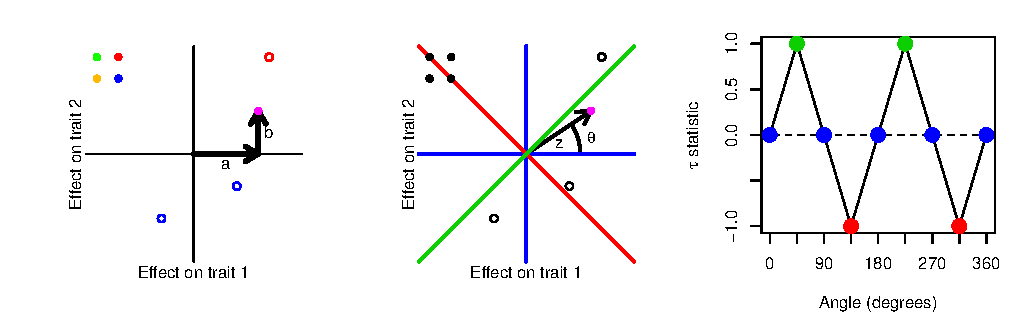
\includegraphics[width=\textwidth]{fig1.eps} % Figure image
    \caption{Measuring pleiotropy. (A) Testing effects on each trait. The effects of eight fictional loci on traits 1 and 2. A reference allele at each locus has effects \textit{a} and \textit{b} on traits 1 and 2 respectively. The grey bars indicate the boundary of statistical significance. Each locus is categorised as affecting zero, one or both traits based on which side of the bars they are located. (B) The same loci, but represented as vectors with angles ($\theta$) and lengths (with length \textit{z}) from the origin. The coloured axes correspond to mechanisms in C. (C) Function $\tau$ relates angles to pleiotropic mechanisms. Three special cases when $\tau$ is -1, 0 or 1 correspond to antagonistic pleiotropy (red), zero pleiotropy (blue) and positive pleiotropy (green) respectively. Values between these points measure everything in between.}
    \label{fig:theory} % Label for referencing with \ref{bear}
\end{figure*}

We consider a biallelic locus associated with two traits typical of many studies.
Those traits may be phenotypes in the same individual (e.g. fecundity, growth rate, survival) or measures of permforance in separate environments (\cite{falconer1952problem}).
The reference allele at this locus has effect $a$ on trait 1 and $b$ on trait 2 (Fig. \ref{fig:theory}A).
We assume that $a$ and $b$ have been estimated appropriately given likely causal relationships between the traits; see \cite*{stephens2013unified} for a detailed discussion.
For most phenotypes $a$ and $b$ would be the difference in phenotype between the reference and alternate alleles.
A notable exception is when the traits are fitness, in which case it is more convenient to use the ratio of $a$ and $b$, reflecting a measure or relative fitness.
It is essential that the distribution of effects on traits 1 and 2 be symmetrical around zero so that the choice of allele is arbitrary, and on the same scale for both traits so they can be compared.
For standard traits this is achieved by subtracting the mean and dividing by the standard deviation before estimating allelic effects.
For ratios this is achieved by taking the log of the ratios.

The next step typically involves some kind of statistical test for the null hypothesis that $a$ or $b$ are zero.
A common approach is to perform two univariate tests for each trait separately, often accompanied by a discussion of the relative direction of the effect on each trait (e.g. \cite{wagner2008pleiotropic, Hall2010, anderson2011life, agren_genetic_2013, ellis2021life}).
Loci that affect both loci are classified as positively or negatively pleiotropic (the green point in Fig. \ref{fig:theory}A), those affecting one trait as showing zero pleiotropy (red and yellow points in Fig. \ref{fig:theory}A), and those affecting neither trait are ignored (blue points in Fig. \ref{fig:theory}A).
We note that other testing variants are available, such as tests for whether a locus affects both or either trait (e.g. \cite{korte2012mixed}; see \cite{porter2017multivariate} for a review and comparison).
Nevertheless, the goal is the same: to classify each locus as affecting one, both, or neither trait via null hypothesis testing.

There are three shortcomings with this approach.
First, by classifying effects based on significance thresholds we ignore useful quantitative information about pleiotropic mechanisms.
For example, if we classify the loci in Fig. \ref{fig:theory}A based on how many traits they each affect we would infer that the green locus affects both traits antagonistic pleiotropy, the red and yellow loci affect one trait, and the blue loci affect neither.
However, it is clear that the filled points are much more similar in their effects to one another (they are all associated with a decrease in trait 1 and an increase in trait 1) than they are to the other points of the same colour.
In this way, simply classifying pleiotropic mechanisms discretises the problem, and ignores the fundamentally quantitative nature of pleiotropy.

Second, it will always be more difficult to find loci associated with two traits than one because it is a priori less likely to find two significant associations than one (\cite{wagner2011pleiotropic, hill2012pleiotropic}).
For a visual intuitiion for this, observe that the light grey regions in Fig. \ref{fig:theory}A corresponding to loci associated with one trait only are much larger than the dark grey regions corresponding to loci associated with two traits. Note that this is intended as a didactic example, and the exact sizes of these regions depend will on the data.
Nevertheless, to a first order approximation and multiple-testing issues notwithstanding, it is generally true that the a priori probability of finding one association is $p=0.05$, but $p^2=0.0025$ for an association with two traits.
This leads to a statistical bias that systematically underestimates the amount of pleiotropy in the system.

Third, use of significance thresholds biases the kinds of effect sizes deemed to be important.
It is well known that, unless sample sizes are large, conditioning on significant associations tends to overestimate effect sizes (\cite{beavis1998qtl, xu2003theoretical}).
This also means we filter out any loci deemed to be 'non-significant'.
The extent to which these matter will depend on the biological question, but quantitative traits that are generally expected to have a substantial contribution from loci with weak to moderate effects, but which can have a substantial contribution to genetic variance *in aggregate* (\cite{Fisher1930}).
Rather than remove them, a stronger approach would be to quantify how much weak effects contribute to overall trade-offs.

In summary, by relying on null-hypothesis testing to infer mechanisms of pleiotropy we (1) discretise what is a continuous phenomenon, (2) underestimate the amount of pleiotropy, and (3) ignore the contribution of weak effects. To alleviate this, we would like a method that (1) quantifies rather than classifies pleiotropic mechanism, (2) focusses on effect sizes and their uncertainty, and (3) uses as much of the data as possible.

\section{Quantifying trade-offs}

\subsection{Effects as angles and magnitudes}

We propose a simple approach to address the goals identified in the previous section.
Rather than define pleiotropic effects along the $x$ and $y$ axes (Fig. \ref{fig:theory}) we instead describe effects as angles and vector lengths.
Without loss of information, any pair of values for $a$ and $b$ can be described via angle $\theta$ and magnitude $z = \sqrt{a^2+b^2}$ (Fig. \ref{fig:theory}B).
$\theta$ is measured (arbitrarily) from the axis pointing right, and contains information about the mechanism of pleiotropy.
When $\theta$ points along the axes in red, blue and green in Fig. \ref{fig:theory}B these correspond to loci showing negative, zero, and positive pleiotropy respectively.
This can be turned into a more useful statistic by taking function $\tau$ of $\theta$ (Fig. \ref{fig:theory}C), which is cyclical and hence must be defined piecewise:
\begin{equation}
\tau=
\begin{cases}
     k\theta, & \text{if}\   0^\circ \geq \theta <  45^\circ \\
   2-k\theta, & \text{if}\  45^\circ \geq \theta < 135^\circ \\
  -2+k\theta, & \text{if}\ 135^\circ \geq \theta < 225^\circ \\
   2+k\theta, & \text{if}\ 225^\circ \geq \theta < 315^\circ \\
  -2+k\theta, & \text{if}\ 315^\circ \geq \theta < 360^\circ
\end{cases}
\end{equation}
where $k=\frac{1}{45}$.
This resembles a linearised sine wave, and is likely to be clearer as a figure (Fig. \ref{fig:theory}C) than an equation.
Values of $\tau$ of -1, 0, and 1 correspond to the special cases of symmetrical negative, zero and positive pleiotropy (red, blue and green in Fig. \ref{fig:theory}B and C).
In addition, all intermediate values between these cases are possible.
In this way, $\tau$ reflects a quantitative measure of the pleiotropic mechanism.

$z$ reflects the overall magnitude of the effect.
Just as larger values of $a$ and $b$ reflect stronger effects on each trait, values of $z$ which are further from the origin reflect a stronger effect overall.
A key difference between these numbers is that $a$ and $b$ measure effects along specific axes, but $z$ but is agnostic about the direction of the effect.
This decouples estimation of the direction and magnitude of the effect.
This also means that estimates of uncertainty can be assessed on one axis only, negating the need to test multiple traits at once.

\subsection{Uncertainty in estimates}

Assess uncertainty by resampling
Parametric,
nonparametric
bayes

How to claculate zstar
get a q

Sometimes you might not be able to do that.
Here's a formula to get a SD on z.

\subsection{\code{sintillate} package}

\section{Application to data}

\subsection{Pleiotropy in local adaptation}

Selection on parental phenotypes

Selection across markers

Somehow relate (mean?) tau to genetic correlation? 

%------------------------------------------------

\section{Discussion}

There is a close correspondence between $\tau$ 
just as genetic correlations of -1, 0 and 1 correspond to negative, zero and positive correlations.

Mention GxE
For examples, reciprocal transplant experiments can uncover adaptation to specific environments between pairs of genotypes or populations \cite{turesson1922, clausen1940experimental, Kawecki2004}.

Stephens 2013
How will errors be correlated if you use different models?

\subsection{Subsection One}

We don't address the question "how many traits?"
Does this extend tp multiple traits?
You could make a G matrix

\subsection{Subsection Two}

\blindtext % Dummy text

%----------------------------------------------------------------------------------------
%	REFERENCE LIST
%----------------------------------------------------------------------------------------

\printbibliography %Prints bibliography

%----------------------------------------------------------------------------------------

\end{document}
